\documentclass[12pt]{article}

\usepackage{graphicx}
\usepackage{paralist}
\usepackage{amsfonts}
\usepackage{listings}
\usepackage{url}
\usepackage{changepage}
\usepackage{makecell}
 %% MIS CODE
 
\usepackage{graphicx}
\usepackage{paralist}
\usepackage{amsfonts}
\usepackage{amsmath}
\usepackage{hhline}
\usepackage{booktabs}
\usepackage{multirow}
\usepackage{multicol}
\usepackage{url}

\oddsidemargin -10mm
\evensidemargin -10mm
\textwidth 160mm
\textheight 200mm
\renewcommand\baselinestretch{1.0}

\newcounter{stepnum}

%% Comments

\usepackage{color}
\usepackage[T1]{fontenc}

\newif\ifcomments\commentstrue

\ifcomments
\newcommand{\authornote}[3]{\textcolor{#1}{[#3 ---#2]}}
\newcommand{\todo}[1]{\textcolor{red}{[TODO: #1]}}
\else
\newcommand{\authornote}[3]{}
\newcommand{\todo}[1]{}
\fi

\newcommand{\wss}[1]{\authornote{blue}{SS}{#1}}

 
 %% MIS CODE 
 
 
\pagestyle {plain}
\pagenumbering{arabic}
 
\begin{document}
%~~~~~~~~~~~~~~~~~~~~~~~  Title  ~~~~~~~~~~~~~~~~~~~~~~~~~~~~~~~~
\begin{titlepage}
    \begin{center}
        \vspace*{1cm}
            
        \Huge
        \textbf{Software Design Document}
 
        \LARGE
        \vspace{0.5cm}
        \textbf{Project Vayu}\\
        \vspace{0.2cm}
        Lab 2, Group 5
 
        \vspace{0.5cm}
        Revision: 0.2\\
        \vspace{0.2cm}
        11 April, 2020
            
        \vspace{1.5cm}
            
        \Large
        Oussama Saoudi, Lennon Yu\\
        Christina Korsman, Diego Soriano
 
        \vfill
            
        \vspace{0.8cm}
                        
        \large
        SFWRENG 2XB3\\
        Software Engineering Practice and Experience:\\
        Binding Theory to Practice\\
        Department of Computing and Software\\
        McMaster University            
    \end{center}
\end{titlepage}
 
\newpage
%~~~~~~~~~~~~~~~~~~~~~~~  Revision  ~~~~~~~~~~~~~~~~~~~~~~~~~~~~~~~~
\Large \noindent \textbf{Change History}\\
\normalsize
\begin{center}
    \begin{tabular}{|| c | c | p{7cm} ||} 
    \hline
    Revision & Date & Changes\\
    \hline\hline
    V0.1 & 27 Feb 2020 & Added skeleton \\ 
    \hline
    V0.2 & 11 April 2020 & Refining details with updated content \\
    \hline
    ~ & ~ & ~ \\
    \hline
    ~ & ~ & ~ \\
    \hline
    ~ & ~ & ~ \\
    \hline
\end{tabular}
\end{center}
 
\Large \noindent \textbf{Team Members}\\
\normalsize
\begin{center}
    \begin{tabular}{|| c | c | l ||} 
    \hline
    Name & Student No. & Role\\
    \hline\hline
    Oussama Saoudi & 400172153 & Project Lead, Search Alg. Dev. \\ 
    \hline
    Lennon Yu & 400183521 & Doc. Maintainer, Graph Alg. Dev. \\
    \hline
    Christina Korsman & 400192880 & Transcriber, FileIO. Dev \\
    \hline
    Diego Soriano & 400172910 & Doc. Maintainer, Sort Alg. Dev. \\
    \hline
\end{tabular}
\end{center}
 
\normalsize
By virtue of submitting this document we electronically sign and date
that the work being submitted by all the individuals in the group is
their exclusive work as a group and we consent to make available the
application developed through SE-2XB3 project, the reports,
presentations, and assignments (not including my name and student number)
for future teaching purposes. 
 
\newpage
%~~~~~~~~~~~~~~~~~~~~~~~  Contribution  ~~~~~~~~~~~~~~~~~~~~~~~~~~~~~~~~
\Large \textbf{Contributions}
\normalsize
\begin{adjustwidth}{-1.2cm}{}
\begin{center}
    \begin{tabular}{| c | c | c | c  || } 
    \hline
    Name & Roles & Contributions & Comments\\
    \hline\hline
     Oussama Saoudi & \makecell{Project Lead,\\Developer} & \makecell{DisasterAreaBuilder, \\ DisasterArea, KdTree,\\ ConvexHull Builder, \\ Quicksort Refinement, Stack, \\ CCFinder Refinement,  \\ DisasterAreaBuilder State \\ Machine} & \makecell{Made \\significant \\refinements to\\ modules to\\ improve \\ performance}\\ 
    \hline
    Lennon Yu & \makecell{Documentation Maintainer,\\ Developer} & \makecell{Graph, CCFinder First Implementation \\ CommandlineController \\ Proofreading SDD MIS} &\\
    \hline
    Christina Korsman & Transcriber, Developer &  \makecell{WeatherTypeEnum, FileOutut, \\ Parse, DisasterType, \\ Meeting Minutes} & \\
    \hline
    Diego Soriano & \makecell{General Programmer, \\Developer} & \makecell{ByDamage, ByProximity, \\Quicksort First Implementation, SRS, SDD} &\\
    \hline
\end{tabular}
\end{center}
\end{adjustwidth}
\newpage
%~~~~~~~~~~~~~~~~~~~~~~~  Summary  ~~~~~~~~~~~~~~~~~~~~~~~~~~~~~~~~
\Large \noindent \textbf{Summary}\\
\normalsize
Project: Vayu is a system which parses NCDC Storm and Weather Events Database to provide a platform on which users can interact with the weather data. This is facilitated through sorting of data points by casualties or by property damage. In addition, the system computes disaster areas which represent areas affected by various weather and disasters. The areas are in the form of sets of points enclosing regions which have high occurrence of a certain weather type. The disaster areas and sorting allow users such as governments or relief organizations to discern useful information about regions affected by certain weather trends or disasters.
 
\newpage
%~~~~~~~~~~~~~~~~~~~~~~~  Table of Content  ~~~~~~~~~~~~~~~~~~~~~~~~~~~~~~~~
\normalsize
\tableofcontents
\newpage
%~~~~~~~~~~~~~~~~~~~~~~~  Body  ~~~~~~~~~~~~~~~~~~~~~~~~~~~~~~~~

% \section{Introduction} 
    
\section{SDD Identification}
    \subsection{Scope}
        The developed product is a program that can read an input set of data from NCDC Storm Events Database, process and translate it into a usable format. The program will be able to sort the given set of disaster data on different parameters, such as casualty count or property damage costs. From this, a graph will be created and used to write a convex hull representation
        of the disaster trends. This information displayed in this format would allow for a better understanding and prediction of natural disaster trends around the globe. The end product aims to serve governments/relief organizations with natural disaster data presented in an easier to process format to help predict further trends.
    \subsection{Purpose}
        The purpose of this document is to provide a description of the software's design and allow a basis from which the software's goals can be referenced to during it's development process. 
    \subsection{Intended Audience}
        The intended audience of this software design descriptions document are governments and relief organizations.
    \subsection{References}
[1]Cengproject.cankaya.edu.tr, 2020. [Online]. Available: http://cengproject.cankaya.edu.tr/wp-content/uploads/sites/10/2017/12/SDD-ieee-1016-2009.pdf. [Accessed: 22- Mar- 2020].
    \subsection{Context}
        The purpose of this software design description is to outline what the software is intended to accomplish as well as the design details of the project as a whole.
    \subsection{Design Languages}
    The Design language that will be use is UML.
    %\subsection{Body}
    %Not necessary?
    %\subsection{Summary}
    %Not necessary?
    %\subsection{Glossary}
    %Not necessary?
        
\section{Design Stakeholders}
    The stakeholder of the design subject with respective design concerns are the following:
    \begin{itemize}
        \item Governments
        \begin{itemize}
            \item Disaster Regions %TODO: LABEL THE CONCERNS
            \item Casualties
          %  \item Severity Indicator
        \end{itemize}
        
        \item Non-profit Organizations
        \begin{itemize}
            \item Disaster Regions %TODO: LABEL THE CONCERNS
            \item Casualties
         %   \item Severity Indicator
        \end{itemize}
        
        \item Insurance Companies
        \begin{itemize}
            \item Property Damage
           % \item Severity Indicator
        \end{itemize}
        
    \end{itemize}

\section{Design Viewpoints}
        \subsection{Context viewpoint}%%all
            The context viewpoint of this software depicts all the services provided by the program.
            \subsubsection{Design concerns}
                The program aims to provide a way to process and present the given input data of natural disasters from the supplied database. Its primary users would be governments and relief organizations, who would analyze trends from the processed data in the use of better natural disaster trend predictions.
            \subsubsection{Design entities}
                The external active elements that the system will be working with, is the user and the data set.
            \subsubsection{Design relationships}
                The system will receive location data , or filter data from the user. With this input the system will out the severity and disaster from the surround area. if applicable the filter on the type of disaster in that area.
            \subsubsection{Design  Constraints}
                %The interaction will be through a %moblie computer application?
                Users interact with it through command line . In terms of quality, a user review is to be given to users after interaction with the program, and an overall positive rating of at least 75\% must be achieved, in accordance with the SRS.
        \subsection{Composition viewpoint}%Lennon
            The composition viewpoint outlines the many components of the software and its subsystems. In-depth explanation of these components and the relations between them will be covered in later sections.
            \subsubsection{Design concerns}
                The design of this programs is structured into modules and sub-modules that interact between different packages. The project as a whole is managed by controlling, editing, and monitoring these components, such as KD-tree, Quicksort, and ConvexHull. Each main function of the program is itself divided into smaller packages, such as those for sorting, searching, and graph management. As a whole, the overall program can be subdivided to equally distribute work amongst the team.
                
            \subsubsection{Design entities}
                A full list of design entities is shown in section 3.3.
            \subsubsection{Design Relationship}
                The design relationship of the program's modules is further explained in section 3.4.
            %\subsubsection{Design attributes}
           % NYI
        \subsection{Interface viewpoint}%Oussama
        The following viewpoint is organized to list the internal and external interfaces of the several modules in the program.
                %//////////////////////////////////////////////////////////////
                %............................................................
                %/////////////////////////////////////////////////////////////
                \newpage
                \subsection* {ByCasualties Module}
                
                \subsubsection*{Template Module inherits Comparator<DisasterPoint>}
                
                ByCasualties
                
                \subsubsection* {Uses}

                None

                \subsection* {Syntax}

                \subsubsection* {Exported Constants}

                None
                
                \subsubsection* {Exported Types}

                ByCasualties = ?

                \subsubsection* {Exported Access Programs}
                
                \begin{tabular}{| l | l | l | p{5cm} |}
                \hline
                \textbf{Routine Name} & \textbf{In} & \textbf{Out} & \textbf{Description}\\
                \hline
                new ByCasualties & & ByCasualties & Constructs a new ByCasualties comparator\\
                \hline
                compare & DisasterPoint, DisasterPoint & int & Compare two DisasterPoints by their casualty numbers, return
                a negative/positive integer or zero if the first DisasterPoint's casualty is less/greater than
                or equal to that of the second DisasterPoint.\\
                \hline
                \end{tabular}
                
                \subsection*{Semantics}

                \subsubsection* {State Variables}

                None
                
                \subsubsection* {State Invariant}

                None
                \subsubsection* {Local Modules}
                
                None
                
                \subsubsection* {Local Functions}
                
                None

                \subsubsection* {Design Concerns}

                ByCasualties allows for comparison between two DisasterPoints relative to the number of casualties stored in each DisasterPoint. This fulfills [FR1.2] which allows for the list of affected areas sorted by casualties.

                %//////////////////////////////////////////////////////////////
                %............................................................
                %/////////////////////////////////////////////////////////////
                \newpage
                \subsection* {ByDamage Module}
                
                \subsubsection*{Template Module inherits Comparator<DisasterPoint>}
                
                ByDamage
                
                \subsubsection* {Uses}

                None

                \subsection* {Syntax}

                \subsubsection* {Exported Constants}

                None
                
                \subsubsection* {Exported Types}

                ByDamage = ?

                \subsubsection* {Exported Access Programs}
                
                \begin{tabular}{| l | l | l | p{5cm} |}
                \hline
                \textbf{Routine Name} & \textbf{In} & \textbf{Out} & \textbf{Description}\\
                \hline
                new ByDamage & & ByDamage & Constructs a new ByDamage comparator\\
                \hline
                compare & DisasterPoint, DisasterPoint & int & Compare two DisasterPoints by their property damage, return
                a negative/positive integer or zero if the first DisasterPoint's property damage is less/greater than
                or equal to that of the second DisasterPoint.\\
                \hline
                \end{tabular}
                
                \subsection*{Semantics}

                \subsubsection* {State Variables}

                None
                
                \subsubsection* {State Invariant}

                None
                
                \subsubsection* {Local Modules}
                
                None
                
                \subsubsection* {Local Functions}
                
                None

                \subsubsection* {Design Concerns}

                This cover the functional requirements [FR 1.1] by comparing the damage of the given area around a point.
        
                %//////////////////////////////////////////////////////////////
                %...........................DisasterPoint.................................
                %/////////////////////////////////////////////////////////////
                \newpage
                \subsection* {Disaster Point Module}
                
                \subsubsection*{Template Module}
                
                DisasterPoint
                
                \subsection* {Uses}
                
                WeatherTypeEnum
                
                \subsection* {Syntax}
                
                \subsubsection* {Exported Constants}
                
                None
                
                \subsubsection* {Exported Types}
                
                DisasterPoint = ?
                
                \subsubsection* {Exported Access Programs}

                \begin{tabular}{| l | l | l | p{5cm} |}
                    \hline
                    \textbf{Routine Name} & \textbf{In} & \textbf{Out} & \textbf{Description}\\
                    \hline
                    new DisasterPoint & $\mathbb{N}$ & DisasterPoint & Constructs a new DisasterPoint with a specified id\\
                    \hline
                    new DisasterPoint & $\mathbb{N}, \mathbb{R}, \mathbb{R}$ & DisasterPoint & Constructs a new DisasterPoint with a specified id, latitude and longitude\\
                    \hline
                    setLat & $\mathbb{R}$ & ~ & Sets the DisasterPoint's latitude \\
                    \hline
                    setLon & $\mathbb{R}$ & ~ & Sets the DisasterPoint's longitude\\
                    \hline
                    setType & WeatherTypeEnum & ~ & Sets the DisasterPoint's disaster type\\
                    \hline
                    setCas & $\mathbb{N}$ & ~ & Sets the DisasterPoint's causalities\\
                    \hline
                    setYear & $\mathbb{N}$ & ~ & Sets the DisasterPoint's year of occurrence\\
                    \hline
                    setPropertyDam & $\mathbb{N}$ & ~ & Sets the DisasterPoint's property damage\\
                    \hline
                    
                    getId & ~ & $\mathbb{N}$ & Gets the DisasterPoint's ID\\
                    \hline
                    getLat & ~ & $\mathbb{R}$ & Gets the DisasterPoint's latitude\\
                    \hline
                    getLon & ~ & $\mathbb{R}$ & Gets the DisasterPoint's longitude\\
                    \hline
                    getWeatherType & ~ & WeatherTypeEnum & Gets the DisasterPoint's disaster type\\
                    \hline
                    getCasualties & ~ & $\mathbb{N}$ & Gets the DisasterPoint's casualties\\
                    \hline
                    getPropertyDamage & ~ & $\mathbb{N}$ & Gets the DisasterPoint's property damage\\
                    \hline
                    getYear & ~ & $\mathbb{N}$ & Gets the DisasterPoint's year of occurrence\\
                    \hline
                    hashCode & ~ & $\mathbb{Z}$ & Returns the hashcode of this DisasterPoint\\
                    \hline
                    equals & DisasterPoint & $\mathbb{B}$ & Checks if two DisasterPoint are equal by ID \\
                    \hline
                    toString & ~ & String & Output the contents of DisasterPoint to a String\\
                    \hline
                    \end{tabular}
                
                \subsection* {Semantics}
                
                \subsubsection* {State Variables}
                    $latitude: \mathbb{R}$\\
                    $longitude: \mathbb{R}$\\
                    $disasterType:$ WeatherTypeEnum\\
                    $year: \mathbb{N}$\\
                    $casualties: \mathbb{N}$\\
                    $propertyDamage: \mathbb{N}$\\
                    $id: \mathbb{N}$\\
                
                \subsubsection* {State Invariant}
                
                None
                
                \subsubsection* {Local Modules}
                
                None
                
                \subsubsection* {Local Functions}
                
                None
                
                \subsubsection* {Design Concerns}
                
                The DisasterPoint module is the most basic data storage entity that is used
                by all modules.
                
                %//////////////////////////////////////////////////////////////
                %............................................................
                %/////////////////////////////////////////////////////////////
                \newpage
                \subsection* {KdTree Module}
                
                \subsubsection*{Template Module}
                
                KdTree
                
                \subsection* {Uses}
                
                DisasterPoint, Stack<T>
                
                \subsection* {Syntax}
                
                \subsubsection* {Exported Constants}
                
                None
                
                \subsubsection* {Exported Types}
                
                KdTree = ?

                \subsubsection* {Exported Access Programs}
                
                % \begin{adjustwidth}{-2cm}{}
                \begin{tabular}{| l | l | l | p{5cm} |}
                    \hline
                    \textbf{Routine Name} & \textbf{In} & \textbf{Out} & \textbf{Description}\\
                    \hline
                    new KdTree & & KdTree & Contructs a new kd-tree\\
                    \hline
                    insert & DisasterPoint & ~ & Inserts a DisasterPoint into the kd-tree\\
                    \hline
                    nearestPoint & DisasterPoint & DisasterPoint & Finds the Nearest point in the KDTree to the given query point and return that point\\
                    \hline
                    closePoints & DisasterPoint, $\mathbb{R}$ & Iterable<DisasterPoint> & Finds all points that are within a certain radius rad from the given query point\\
                    \hline
                \end{tabular}
                % \end{adjustwidth}
                \subsection* {Semantics}
                
                \subsubsection* {State Variables}
                
                $root:$ KdTree.Node\\
                    
                \subsubsection* {State Invariant}
                
                None
                
                \subsubsection* {Local Modules}
                
                \begin{itemize}
                    \item[KdTree.Node] DisasterPoint object representing node in the kd binary tree with 
                                	   representative point in 2d space, an orientation, showing
                                	   if its dividing line is horizontal or vertical. DisasterPoint also has a
                                	   left or right node, which could also represent up or down if its
                                	   line is horizontal. RectA inside node represents the Rectangle it 
                                	   sits in and divides.
                    \item[KdTree.RectA] Rectangular Area data type which represents area in
	                                    2D space with minimum and maximum x and y values.
                \end{itemize}
                
                \subsubsection* {Local Functions}
                
                \noindent Node insert(Node node, DisasterPoint p, boolean orientation, double xmin, double ymin, double xmax, double ymax):
			    \begin{itemize}
			        \item Inserts the DisasterPoint p at the kdTree by analyzing the node and orientation
                	 to find placement of the point. xmin, ymin, xmax, and ymax represent the bounds
                	 of the area being checked by the kdtree for the position to place the point.
                	 When the new node is made with its associated point, it will occupy a RectA area
                	 with bounds xmin, ymin, xmax, and ymax.
			    \end{itemize}
			    
                \noindent int size(Node n):
			    \begin{itemize}
			        \item Returns the size of the node's subtree if it is not null, else returns 0
			    \end{itemize}
			    
                \noindent int compareX(DisasterPoint p1, DisasterPoint p2):
			    \begin{itemize}
			        \item Compares the x value between two DisasterPoints p1 and p2.
                	 Returns 1 if p1 has greater x value, returns -1 if p2 has
                	 greater value, and 0 otherwise.
			    \end{itemize}
			    
                \noindent int compareY(DisasterPoint p1, DisasterPoint p2):
			    \begin{itemize}
			        \item Compares the y value between two DisasterPoints p1 and p2.
                	 Returns 1 if p1 has greater y value, returns -1 if p2 has
                	 greater value, and 0 otherwise.
			    \end{itemize}
			    
                \noindent DisasterPoint nearestPoint(Node node, DisasterPoint query, DisasterPoint nearestPoint):
			    \begin{itemize}
			        \item Finds the nearest point in the kdTree to the query DisasterPoint.
			    \end{itemize}
			    
                \noindent void range(Node node, RectA rect, Stack<DisasterPoint> stack):
			    \begin{itemize}
			        \item Finds all DisasterPoints existing in the RectA rectangle passed to the method
			    \end{itemize}
                
                \subsubsection* {Design Concerns}
                It assists in creating connections to the graph, which facilitates the creation of disaster regions for
                functional requirements [FR2.1] and [FR5.3]
                
                %//////////////////////////////////////////////////////////////
                %............................................................
                %/////////////////////////////////////////////////////////////
                 \newpage
                \subsection* {Quicksort Module}
                
                \subsubsection*{Module}
                
                Quicksort
                
                \subsection* {Uses}
                
                None
                
                \subsection* {Syntax}
                
                \subsubsection* {Exported Constants}
                None
                \subsubsection* {Exported Types}
                None
                \subsubsection* {Exported Access Programs}
                \begin{tabular}{| l | l | l | p{5cm} |}
                    \hline
                    \textbf{Routine Name} & \textbf{In} & \textbf{Out} & \textbf{Description}\\
                    \hline
                     sort            & List<T> , Comparator<T> & ArrayList<T> & Copies and sorts list of type T, and returns the copy. Uses comparator c
                     to compare values in the list. \\
                    \hline
                     sort            & List<T> , $\mathbb{N}, \mathbb{N}$, Comparator<T>    &ArrayList<T> & Copies and sorts list of type T with a given starting and ending index, and returns the copy. Uses comparator c
                     to compare values in the list. \\
                    \hline
                     quicksort       &ArrayList<T>, $\mathbb{N}, \mathbb{N}$,Comparator<T> &       ~  & Performs quicksort by partitioning the list and recursively sorting the sub lists. Modifies the given list directly.\\
                    \hline
                \end{tabular}
                    
                \subsection* {Semantics}
                
                \subsubsection* {State Variables}
                
                \subsubsection* {State Invariant}
                None
                
                \subsubsection*{Local Modules}
                
                None
                
                \subsubsection*{Local Functions}
                
                \noindent int partitionRandom(ArrayList<T> list, int lo, int hi, Comparator<T> c):
			    \begin{itemize}
			        \item Switches the first value in a sublist with a random value in that sublist to improve sorting performance
			    \end{itemize}
                \noindent int partition(List<T> list,int lo, int hi, Comparator<T> c):
			    \begin{itemize}
			        \item Partitions values in a list into values less than the first item in the list and
	                elements greater than the the first element
			    \end{itemize}
                \noindent void exch(List<T> list, int i1, int i2):
			    \begin{itemize}
			        \item Exchanges two values in a list at indexes i1 and i2
			    \end{itemize}
			
                \subsubsection* {Design Concerns}
                
                It fulfills [FR 1.1] which enables sorting all disaster points either by property damage or casualties.
                
                %//////////////////////////////////////////////////////////////
                %............................................................
                %/////////////////////Christina ////////////////////////////////////////
                \newpage
                \subsection* {Connected Component Finder Module}
                
                \subsubsection*{Template Module}
                
                CCFinder
                
                \subsection* {Uses}
                
                Graph
                
                \subsection* {Syntax}
                
                \subsubsection* {Exported Constants}
                
                None

                \subsubsection* {Exported Types}
                
                CCFinder = ?

                \subsubsection* {Exported Access Programs}
                
                
                \begin{tabular}{| l | l | l | p{5cm} |}
                \hline
                \textbf{Routine name} & \textbf{In} & \textbf{Out} & \textbf{Description}\\
                \hline
                new CCFinder & Graph & CCFinder & Constructs a new Connected Component Finder\\
                \hline
                connected&$\mathbb{N}, \mathbb{N}$& $\mathbb{B}$ & Checks if two vertices are in the same component (i.e. a path exists between two vertices)\\
                \hline
                componentCount & ~ & $\mathbb{N}$ & Gets the number of existing connected components. One may assume that all component id's are less than this value.\\
                \hline
                getComponentById &$\mathbb{N}$ &HashSet<Integer>&Gets a connected component by its id\\
                \hline 
                toString&~&String&String representation of CCFinder\\
                \hline
                \end{tabular}
                
                \subsection* {Semantics}
                    \subsubsection* {State Variables}
                    
                    \textit{componentCount}: $\mathbb{N}$\\
                    \textit{marked}: sequence of $\mathbb{B}$\\
                    \textit{id}: sequence of $\mathbb{N}$\\
                    \textit{components}: ArrayList<HashSet<Integer> >\\
                        
                    \subsubsection* {State Invariant} None
                
                \subsubsection*{Local Modules}
                
                None
                
               \subsection*{Local Functions}
                   \noindent dfs(Graph G, int s):
                    \begin{itemize}
                        \item Performs depth first search in the graph G starting from source s. Adds all the explored points to a connected component

                    \end{itemize}
                    \noindent validPoint(int v):
                    \begin{itemize}
                        \item Checks if the passed integer vertex is in the graph. If it isn't throws IllegalArgumentException.

                    \end{itemize}
                    
                \subsubsection* {Design Concerns}
                Required by DisasterAreaBuilder module to construct proper convex hulls [FR 2.1].
                %//////////////////////////////////////////////////////////////
                %............................................................
                %/////////////////////////////////////////////////////////////Christina
                \newpage
                \subsection* {Graph Module}
                \subsubsection*{Template Module}
                
                Graph 
                
                \subsection* {Uses}
                
                None
                
                \subsection* {Syntax}
                \subsubsection* {Exported Constants}
                None
                
                \subsubsection* {Exported Types}
                
                Graph = ?
                
                \subsubsection* {Exported Access Programs}
                
                \begin{tabular}{| l | l | l | p{5cm} |}
                \hline
                \textbf{Routine name} & \textbf{In} & \textbf{Out} & \textbf{Description}\\
                \hline
                new Graph& $\mathbb{N}$ & Graph &  Constructs a new graph\\
                \hline
                 addEdge & $\mathbb{N}, \mathbb{N}$ & ~ & Connect two vertices in the graph with a new undirected edge.\\
                \hline
                 adj & $\mathbb{N}$ & Iterable<Integer>  & Gets the adjacent vertices of a specific vertex\\
                \hline
                 V & ~ & $\mathbb{N}$ & Gets the number of vertices in this graph\\
                \hline
                 E & ~ & $\mathbb{N}$ & Gets the number of edges in this graph\\
                \hline
                 degree & $\mathbb{N}$ & $\mathbb{N}$ & Gets the number of edges of a specific vertex\\
                \hline
                 toString & ~ & String &  Gets the string representation of this graph\\
                \hline
                \end{tabular}
                
                \subsection* {Semantics}
                    \subsubsection *{State Variables} 
                        $V: \mathbb{N}$\\
                        $E : \mathbb{N}$\\
                        $adj:$  ArrayList<Integer>[]
                    \subsubsection *{State Invariant}
                    
                    None
                    
                     \subsubsection* {Local Modules}
                     None
                
                \subsubsection*{Local Functions}
                
                \noindent void validPoint(int v):
			    \begin{itemize}
			        \item Checks if the passed integer vertex is in the graph. If it isn't throws IllegalArgumentException.
			    \end{itemize}
			    
                    \subsubsection*{Consideration}
                    This module is required by the ConvexHullBuilder and KdTree modules in the completion of their functional requirements [FR 2.1]
                   \newpage
                %//////////////////////////////////////////////////////////////
                %............................................................
                %/////////////////////Christina ////////////////////////////////////////
                 \newpage
                \subsection* {Weather Type Enum Module}
                
                \subsubsection*{Template Module}
                
                WeatherTypeEnum
                
                \subsection* {Uses}
                
                None
                
                \subsection* {Syntax}
                
                \subsubsection* {Exported Constants}
                
                None
                
                \subsubsection* {Exported Types}
                DisasterTypes = \{Astronomical Low Tide, Avalanche, Blizzard, Coastal Flood, Cold/Wind Chill, Debris Flow, Dense Fog, 
                Dense Smoke, Drought, Dust Devil, Dust Storm, Excessive Heat, Extreme Cold/Wind Chill, Flash Flood, Flood,Frost/Freeze,
                Funnel Cloud, Freezing Fog, Hail, Heat, Heavy Rain, Heavy Snow, High Surf, High Wind, Hurricane(Typhoon),Ice Storm, 
                Lake-Effect Snow, Lake shore Flood,Lighting, Marine Hail, Marine High Wind, Marine Strong Wind, Marine Thunder Wind, 
                Rip Current, Seiche, Sleet, Storm Surge/Tide, Strong Wind, Thunderstorm Wind, Tornado, Tropical Depression, Tropical Storm
                Tsunami, Volcanic Ash, Waterspout , Wildfire, Winter Storm, Winter Weather  \}\\
                         
                \subsubsection* {Exported Access Programs}
                
                % \begin{adjustwidth}{-1cm}{}
                \begin{tabular}{| l | l | l | p{5cm} |}
                \hline
                \textbf{Routine name} & \textbf{In} & \textbf{Out} & \textbf{Description}\\
                \hline
                new WeatherTypeEnum & String & WeatherTypeEnum & Constructs WeatherTypeEnum from associated text.\\
                \hline
                 getText & ~ & String & Returns the associated name of the WeatherTypeEnum\\
                \hline
                 fromString & String & WeatherTypeEnum & Returns the WeatherTypeEnum associated with the given text if it exists, else return null.\\
                \hline
                \end{tabular}
                % \end{adjustwidth}
                \subsection* {Semantics}
                    \subsubsection *{State Variables} None
                    \subsubsection *{State Invariant} None
                    
                     \subsubsection* {Local Modules}
                     None
                
                \subsubsection*{Local Functions}
                None
                    
                \subsubsection *{Considerations}
                The types enumerates over all the disaster types in the input data file. It is required by all modules to select a particular disaster type in real life.
                \newpage
               
                %//////////////////////////////////////////////////////////////
                %............................................................
                %/////////////////////////////////////////////////////////////Christina
                \subsection* {Disaster Area Module}
                
                \subsubsection*{Template Module}
                
                DisasterArea
                
                \subsection* {Uses}
                
                DisasterPoint, WeatherTypeEnum
                
                \subsection* {Syntax}
                
                \subsubsection * {Exported Constants}
                
                None
                
                \subsubsection* {Exported Types}
                
                DisasterArea = ?
                
                \subsubsection* {Exported Access Programs}
                
                %  \begin{adjustwidth}{-1cm}{}
                \begin{tabular}{| l | l | l | p{5cm} |}
                \hline
                \textbf{Routine name} & \textbf{In} & \textbf{Out} & \textbf{Description}\\
                \hline
                new DisasterArea & \makecell{ArrayList<DisasterPoint>, \\ ArrayList<DisasterPoint>, \\ WeatherTypeEnum} & DisasterArea & Constructor for DisasterArea which takes in the area's convex hull, all the DisasterPoints contained within the convex hull, and the shared weather type of all the nodes\\
                \hline 
                getType&~&WeatherTypeEnum&Getter for the WeatherTypeEnum of the DisasterArea\\
                \hline
                getHull&~&ArrayList<DisasterPoint>&Gets the convex hull of the DisasterPoints contained in the DisasterArea\\
                \hline
                getAllNodes&~&ArrayList<DisasterPoint>&Gets all the nodes contained in the DisasterArea\\
                \hline
                \end{tabular}
                % \end{adjustwidth}
                
                \subsection* {Semantics}
                    \subsubsection *{State Variables} 
                        $convexHull:$ ArrayList<DisasterPoint>\\
                        $allNodes:$ ArrayList<DisasterPoint>\\
                        $disasterType:$ WeatherTypeEnum \\
                       
                    \subsubsection *{State Invariant}
                    
                    None
                    
                    \subsubsection*{Local Modules}
                    
                    None
                    
                    \subsubsection*{Local Functions}
                    
                    None
                    
                    \subsubsection*{Consideration}
                    
                    This module is used to cover the functional requirements [FR2.1]
                    
                   \newpage
                 %//////////////////////////////////////////////////////////////
                %............................................................
                %/////////////////////////////////////////////////////////////
                \subsection* {Disaster Area Builder Module}
                
                \subsubsection*{Template Module}
                
                DisasterArea
                
                \subsection* {Uses}
                
                DisasterPoint, WeatherTypeEnum, DisasterArea, Graph, CCFinder, KdTree, ConvexHullBuiler
                
                \subsection* {Syntax}
                
                \subsubsection * {Exported Constants}
                
                None
                
                \subsubsection* {Exported Types}
                
                DisasterAreaBuilder = ?
                
                \subsubsection* {Exported Access Programs}
                
                %\begin{adjustwidth}{-1cm}{}
                \begin{tabular}{| p{3cm} | p{5cm} | l | p{5cm} |}
                \hline
                \textbf{Routine name} & \textbf{In} & \textbf{Out} & \textbf{Description}\\
                \hline
                new DisasterAreaBuilder&Hashtable<Integer,Integer>, ArrayList<DisasterPoint>, $\mathbb{R}, \mathbb{Z}$&  DisasterAreaBuilder      &Builds all the disaster areas on the map. The radius rad is for search of nearest nodes when connecting close DisasterPoints. The minimum size of a disaster area can be specified using the method parameter thresh\\
                \hline
                getAreas&WeatherTypeEnum&ArrayList<DisasterArea>&Returns list of all the DisasterAreas which have a the passed weather type type.\\
                \hline
                \end{tabular}
                %\end{adjustwidth}
                \subsection* {Semantics}
                    \subsubsection *{State Variables} 
                      $ kdtList$: Hashtable<WeatherTypeEnum, KdTree>\\
                      $pointList$: ArrayList<DisasterPoint> \\
                      $areaList$: HashMap<WeatherTypeEnum,ArrayList<DisasterArea> >\\
                       
                    \subsubsection *{State Invariant}
                    
                    None
                    
                    \subsubsection* {Local Modules}
                    
                     None
                
                \subsubsection*{Local Functions}
                
                \noindent ArrayList<DisasterPoint> convertToPoint(Iterable<Integer> iterable):
			    \begin{itemize}
			        \item Converts an iterable of integers into a list of DisasterPoints, using the integers as indices in the arrays and returns the list.
			    \end{itemize}
			    
		        \subsubsection*{Consideration}
		        
                This module is used to cover the functional requirements [FR2.1]
                  
                \newpage

                   
                %/////////////////////////////////////////////////////////////
                %...............DIEGODIEGODIEGODIEGODIEGODIEGODIEGODIEGO.......
                %/////////////////////////////////////////////////////////////
                \newpage
                %//////////////////////////////////////////////////////////////
                %...................Parser.........................................
                %/////////////////////////////////////////////////////////////
                \subsection* {File Parser Module}
                
                \subsubsection*{Template Module}
                
                Parser
                
                \subsection* {Uses}
                
                WeatherTypeEnum, DisasterPoint
                
                \subsection* {Syntax}
                
                \subsubsection*{Exported Constants}
                
                \subsubsection* {Exported Types}
                
                Parser = ?
                
                \subsubsection* {Exported Access Programs}
                % \begin{adjustwidth}{-1cm}{}
                \tabcolsep=0.05cm
                \begin{tabular}{| l | l | l | p{11cm} |}
                \hline
                \textbf{Routine name} & \textbf{In} & \textbf{Out} & \textbf{Description}\\
                \hline
                new Parser & ~ & Parser & Initializes parsing of the input files and creation of DisasterPoints\\
                \hline
                detailsParser & String & ~ & Parses given file with name fileName, and creates DisasterPoints from data. Adds all the created DisasterPoints to a the nodeList\\
                \hline
                getData & ~ & ~ & Returns the ArrayList of DisasterPoints created and stored by the parser\\
                \hline
                getTable & ~ & ~ & Getter for the hash table constructed by parser to map id of Disasterpoint to its index\\
                \hline
                \end{tabular}
                
                \subsection* {Semantics}
                
                \subsubsection *{State Variables} 
                
                    \textit{lookup}: Hashtable<Integer,Integer>\\
                    \textit{nodelist}: ArrayList<DisasterPoint>\\

                \subsubsection *{State Invariant}
                
                None
                
                \subsubsection*{Local Modules}
                
                None
                
                \subsubsection*{Local Functions}
                
                \noindent void parse():
                \begin{itemize}
                    \item Sets the base directory for all the files to be parsed
                \end{itemize}
                
                \noindent void getFiles(File dir):
                \begin{itemize}
                    \item Gets all the files in the given directory dir and runs the detailsParser
	                    on files that are not directories. If a directory is contained in dir, it
	                    recursively searches by called getFiles on that directory.
                \end{itemize}
                
                \noindent void detailsParser(String fileName):
                \begin{itemize}
                    \item Parses given file with name fileName, and creates DisasterPoints from data.
                    Adds all the created DisasterPoints to a the nodeList
                \end{itemize}
                
                \noindent int sumCasualties(String injuryD, String injuryI, String deathD, String deathI):
                \begin{itemize}
                    \item Takes 4 strings which are each representing integers for injuries and deaths,
                    converts them to integer, and returns the sum of all the integers.
                \end{itemize}
                
                \noindent int damageParse(String pDamage, String cDamage):
                \begin{itemize}
                    \item Takes string representation of  property damage and crop damage and
                    converts to Double, then returns their sum
                \end{itemize}
                
                \subsubsection*{Consideration}
                
                This module converts data entries in ASCII character based CSV files to corresponding
                programming entities (i.e. DisasterPoint module instances).
                
                
                % \end{adjustwidth}
                
                %//////////////////////////////////////////////////////////////
                %............................................................
                %/////////////////////////////////////////////////////////////
                %//////////////////////////////////////////////////////////////
                %...............DIEGODIEGODIEGODIEGODIEGODIEGODIEGODIEGO.......
                %/////////////////////////////////////////////////////////////
                \newpage
                %//////////////////////////////////////////////////////////////
                %............................................................
                %/////////////////////////////////////////////////////////////
                \subsection* {File Output Module}
                
                \subsubsection*{Template Module}
                
                FileOutput
                
                \subsection* {Uses}
                
                DisasterPoint, DisasterArea
                
                \subsection* {Syntax}
                
                \subsubsection* {Exported Types}
                
                FileOutput = ?
                
                \subsubsection* {Exported Access Programs}
                
                
                \begin{tabular}{| l | l | l | p{5cm} |}
                \hline
                \textbf{Routine name} & \textbf{In} & \textbf{Out} & \textbf{Description}\\
                \hline
                new FileOutput & ~ & ~ & Initializes the FileOutput and creates the line separator which separates the DisasterPoints when being printed\\
                \hline
                writeData & String, ArrayList$<$DisasterPoint$>$ & ~ & Writes data to a file with the same name as the String. Every line on that file is a new DisasterPoint, and in each line, separated by commas, are the attributes of that DisasterPoint.\\
                \hline
                writeAreas & String, ArrayList$<$DisasterArea$>$ & ~ & Writes Data to a file with the same name as the String. Every line on that file is a new DisasterArea, and in each line, separated by commas, are the attributes of the WeatherTypeEnum.\\
                \hline
                \end{tabular}
                
                \subsection* {Semantics}
                
                \subsubsection *{State Variables} 
                
                    \textit{sep}: String\\
                    \textit{numOfFields}: $\mathbb{N}$\\
                    \textit{sizeOfField}: $\mathbb{N}$\\
                    
                \subsubsection *{State Invariant}
                
                None
                
                \subsubsection*{Local Modules}
                
                None
                
                \subsubsection*{Local Functions}
                
                None
                
                \subsubsection* {Design Concerns}

                This module takes the outputs from the Quicksort module and inputs it in a textfile for the users to use.
                This module fulfills the functional requirements [FR3.1] and [FR3.2] by outputting the information into a text file with CSV (Comma Separated Value) in the file.
                %//////////////////////////////////////////////////////////////
                %............................................................
                %/////////////////////////////////////////////////////////////
                %//////////////////////////////////////////////////////////////
                %...............DIEGODIEGODIEGODIEGODIEGODIEGODIEGODIEGO.......
                %/////////////////////////////////////////////////////////////
                \newpage
                %//////////////////////////////////////////////////////////////
                %............................................................
                %/////////////////////////////////////////////////////////////
                \subsection* {Convex Hull Builder Module}
                
                \subsubsection*{Module}
                
                ConvexHullBuilder
                
                \subsection* {Uses}
                
                DisasterPoint, Quicksort, Stack<T>
                
                \subsection* {Syntax}
                
                \subsubsection* {Exported Types}
                
                None
                
                \subsubsection* {Exported Access Programs}
                
                % \begin{adjustwidth}{-1.25cm}{}
                \begin{tabular}{| l | l | l | p{5cm} |}
                \hline
                \textbf{Routine name} & \textbf{In} & \textbf{Out} & \textbf{Description}\\
                \hline
                convexHull & ArrayList<DisasterPoint> & ArrayList<DisasterPoint> & Computes the convex hull of the list of points provided. ie; it computes the smallest set of points when if connected as a polygon contain all the points in the input set DisasterPoints\\
                \hline
                \end{tabular}
                % \end{adjustwidth}
                \subsection*{Semantics}
                
                \subsubsection*{State Variables}
                
                None
    
                \subsubsection* {Local Modules}
                
                \begin{itemize}
                    \item[ConvexHullBuilder.PointComparator] A Comparator for comparing points based off angle to a given anchor DisasterPoint. Used in performing Graham Scan algorithm.
                \end{itemize}
                
                \subsubsection* {Local Functions}
                
                \noindent DisasterPoint nextToTop(Stack<DisasterPoint> pointStack):
                \begin{itemize}
                    \item Returns the second to the top item in the pointStack. The item has a type DisasterPoint.
                \end{itemize}
                
                \noindent void exch(ArrayList<DisasterPoint> disasterPoints, int p1, int p2):
                \begin{itemize}
                    \item Exchanges Points in the two array positions array[p1] and array[p2]
                \end{itemize}
                
                \noindent int orientation(DisasterPoint p1, DisasterPoint p2, DisasterPoint p3):
                \begin{itemize}
                    \item Checks if points p1, p2, and p3 have a clockwise, collinear, or counterclockwise orientation. If they are in a counter clock-wise orientation, returns 2, clock-wise returns 1 and collinear returns 0.
                \end{itemize}
                
                \subsubsection*{Considerations}
                
                This module fulfills functional requirement [FR 2.1].
                
                %//////////////////////////////////////////////////////////////
                %............................................................
                %/////////////////////////////////////////////////////////////
                 %//////////////////////////////////////////////////////////////
                %............................................................
                %/////////////////////////////////////////////////////////////
                \newpage
                 \subsection* {Stack Module}
                
                \subsubsection*{Generic Template Module inherits Iterable<T>}
                
                Stack<T>
                
                \subsection* {Uses}
                
                None
                
                \subsection* {Syntax}
                \subsubsection * {Exported Constants}
                
                None
                
                \subsubsection* {Exported Types}
            
                Stack<T> = ?
                
                \subsubsection* {Exported Access Programs}
                
                
                \begin{tabular}{| l | l | l | p{5cm} |}
                \hline
                \textbf{Routine name} & \textbf{In} & \textbf{Out} & \textbf{Description}\\
                \hline
                new Stack &  & Stack & Constructs a new empty stack\\
                \hline 
                 iterator & ~ & Iterator<T> & Returns iterator for all values in the stack\\
                \hline 
                isEmpty& ~ & $\mathbb{B}$ & Returns true if stack is empty and false otherwise.\\
                \hline 
                size& ~ &$\mathbb{N}$ &returns number of values in the stack\\
                \hline 
                push& T & ~ &Pushes item to the top of the stack\\
                \hline
                pop & ~ & T & Deletes the item on the top of the stack and returns it\\
                \hline
                top& ~ & T &Returns the top item in the stack without popping it\\
                \hline
                \end{tabular}
                \subsection* {Semantics}
                    \subsubsection *{State Variables} 
                        \textit{first}: Node\\
                        \textit{numberOfValues}: $\mathbb{N}$
                    \subsubsection *{State Invariant} None
                    
                    \subsubsection* {Local Modules}
                
                \begin{itemize}
                    \item[Stack.ListIterator] Implements an iterator for Items, which allows for proper iteration through the stack structure.
                    \item[Stack.Node] Node class which stores generic item and next node.
                \end{itemize}
                
                \subsubsection* {Local Functions}
                
                None
                    
                \subsubsection*{Consideration} This module is required by the ConvexHullBuilder and KdTree modules in the completion of their functional requirements.
                    
                \subsubsection*{Considerations}    
                
                The Stack<T> module is used by several other modules to provide the most rudimentary algorithmic functionalities.
                
        \newpage
        
          %//////////////////////////////////////////////////////////////
          %............................................................
           %/////////////////////////////////////////////////////////////
           
           \newpage
                 \subsection* {CommandlineController Module}
                
                \subsubsection*{Template Module}
                
                CommandlineController
                
                \subsection* {Uses}
                
                Parser, FileOutput, DisasterAreaBuilder, WeatherTypeEnum, Quicksort
                
                \subsection* {Syntax}
                \subsubsection * {Exported Constants}
                
                None
                
                \subsubsection* {Exported Types}
            
                CommandlineController = ?
                
                \subsubsection* {Exported Access Programs}
            
                \begin{tabular}{| l | l | l | p{5cm} |}
                \hline
                \textbf{Routine name} & \textbf{In} & \textbf{Out} & \textbf{Description}\\
                \hline
                new CommandlineController &  & CommandlineController & ~\\
                \hline 
                start & ~ & ~ & Starts the user interface\\
                \hline 
                \end{tabular}
                
                \subsection* {Semantics}
                
                \subsubsection *{State Variables} 
                
                    \textit{parser}: Parser\\
                    \textit{DAbuilder}: DisasterAreaBuilder\\
                    \textit{outputter}: FileOutput\\
                    
                \subsubsection *{State Invariant}
                
                None
                
                \subsubsection*{Local Modules}
                
                None
                
                \subsubsection*{Local Functions}
                
                \noindent void performNextCommand():
			    \begin{itemize}
			        \item Takes user input and performs command based on the input
			    \end{itemize}
                
                \noindent void printHelp(String[] args):
			    \begin{itemize}
			        \item Prints help information, depending on the user input prints information on the sort command or the areas command
			    \end{itemize}
                
                \noindent void printHelpSort():
			    \begin{itemize}
			        \item Prints the help for the sort function
			    \end{itemize}
                
                \noindent printHelpAreas():
			    \begin{itemize}
			        \item Prints the help for the areas function
			    \end{itemize}
                
                \noindent void printNoMatch():
			    \begin{itemize}
			        \item Prints if no match to the command input by user is found
			    \end{itemize}
                
                \noindent sort(String[] args):
			    \begin{itemize}
			        \item Initializes the sort command, with the input being the user's arguments for the type of sorting and output file
			    \end{itemize}
                
                \noindent void areas(String[] args):
			    \begin{itemize}
			        \item Initializes the areas command, with the input being the user's arguments for the type of sorting and output file
			    \end{itemize}
                
                \noindent WeatherTypeEnum enumOfString(String rpr):
			    \begin{itemize}
			        \item Takes string rpr and returns the corresponding WeatherTypeEnum which is associated with that string
			    \end{itemize}
                
                \noindent void exit(int exitCode):
			    \begin{itemize}
			        \item Exits from the program with the given exitCode
			    \end{itemize}
                
                \noindent void close():
			    \begin{itemize}
			        \item Closes the input scanner used in the command line8
			    \end{itemize}
		    
                \subsubsection*{Consideration}
                
                This module helps with fulfilling functional requirement [FR 4.2].
                
        \newpage
        
          %//////////////////////////////////////////////////////////////
          %............................................................
           %/////////////////////////////////////////////////////////////
                
    %%%%%%%%%%%%%%%%%%%%%%%%%%%%%%%%%%%%%%%%%%%%%%%%%%%%%%%%%%%%%%%%%%%%%%%%%%%%%%%%%%%%%%%%%%%%%%%%
        
        \subsection{Dependency viewpoint}%Diego
            
            \subsubsection{Design concerns}
            The concerns of this viewpoint are the relationships between the components in the program. This allows maintainers to see the overall structure of the program as a series of interconnected modules, which will allow an overall easier process in the location and isolation of modules creating errors or problems.
            
            \subsubsection{Design entities, relations, and attributes}
            A full list of the dependencies of this program can be found in section 3.6.
        
        \subsection{Information viewpoint}%Christina
            \subsubsection{Design concerns}
                Concerns of this viewpoint are the persistent data structures. The way that this will be address is that the data will be stored in a Graph. This covers the functional requirements [FR2.1], [FR2.1]
            
            \subsubsection{Design entities}
                %data items, data types , classes, data stores , access mechanism 
                 Modules 
                \begin{itemize}
                    \item QuickSort - A module that implements the quick sort algorithm on the graph 
                    \item Casualties Comparator - A module compare the casualties of two disasters 
                    \item Property Damage Comparator - A module compare the property damage of two disasters 
                    \item DisasterPoint - A class that store the data relating to a disaster occurrence. 
                    \item Weather Type Enum - A Data type for all type of disasters in the data set
                    \item Parser -Take the file and transfers the data to another class to be used 
                   % \item File Output - The result of the user interacting with the program. It is an interface
                    \item Graph - A graph data structure 
                    \item Connected Components Finder (Algorithm)- A module that implements algorithm that finds connected components on the Graph
                    \item Convex Hull finder(Algorithm) -A module that implements an algorithm that finds the convex hull on the graph
                    \item Convex Hull - A module that implements the Convex Data structure 
                    \item KD-Tree (Data Structure)- A module that implements the KD- Tree Data structure 
                   % \item GUI- 
                \end{itemize}
                
            \subsubsection{Design relationships}
                \begin{itemize}
                    \item Quicksort use the DisasterPoint class as it the object type to be sorted.
                    \item Causalities Comparator will use DisasterPoint. It will use the getter methods to allow the comparison 
                    \item Property Damage Comparator will use DisasterPoint. It will use the getter methods to allow the comparison
                    \item Promitiy Comparator will use DisasterPoint. It will use the getter methods to allow the comparison 
                    \item DisasterPoint use Enum for the disaster type that it will store for that occurrence 
                   % \item File Output use Filter to make a list of disaster of the filter input types. 
                    \item Filter use Weather Type to apply the filter to be used.
                    \item Graph class use the DisasterPoint class to create a graph data structure 
                    \item Parser use DisasterPoints, taking data and separating it into the correct places for the DisasterPoint.
                    \item finder use Graph and Convex Hull
                    
                    \item Convex hull will use graph 
                    %i have no idea how it will be implemented 
                    \item KD -tree will use graph 
                \end{itemize}
                
            \subsubsection{Design Attributes}
                %persistence and quality properties
                DisasterPoint will be persistently use through out this software,as it is the main container for the data.
                
       % \subsection{Patterns use viewpoint}%Lennon
    %        Summary of patterns use viewpoint here.
    %        \subsubsection{Design concerns}
                
    %        \subsubsection{Design entities}
    %        NYI
    %        \subsubsection{Design relationships}
    %        NYI
    %        \subsubsection{Design Attributes}
    %        NYI
    %        \subsubsection{Design  Constraints}
    %        NYI
            
        % interface will be done after all modules are completed 
        \subsection{Logical viewpoint}%Christina or Diego
         %input UML diagram here 
        \noindent \begin{figure}
            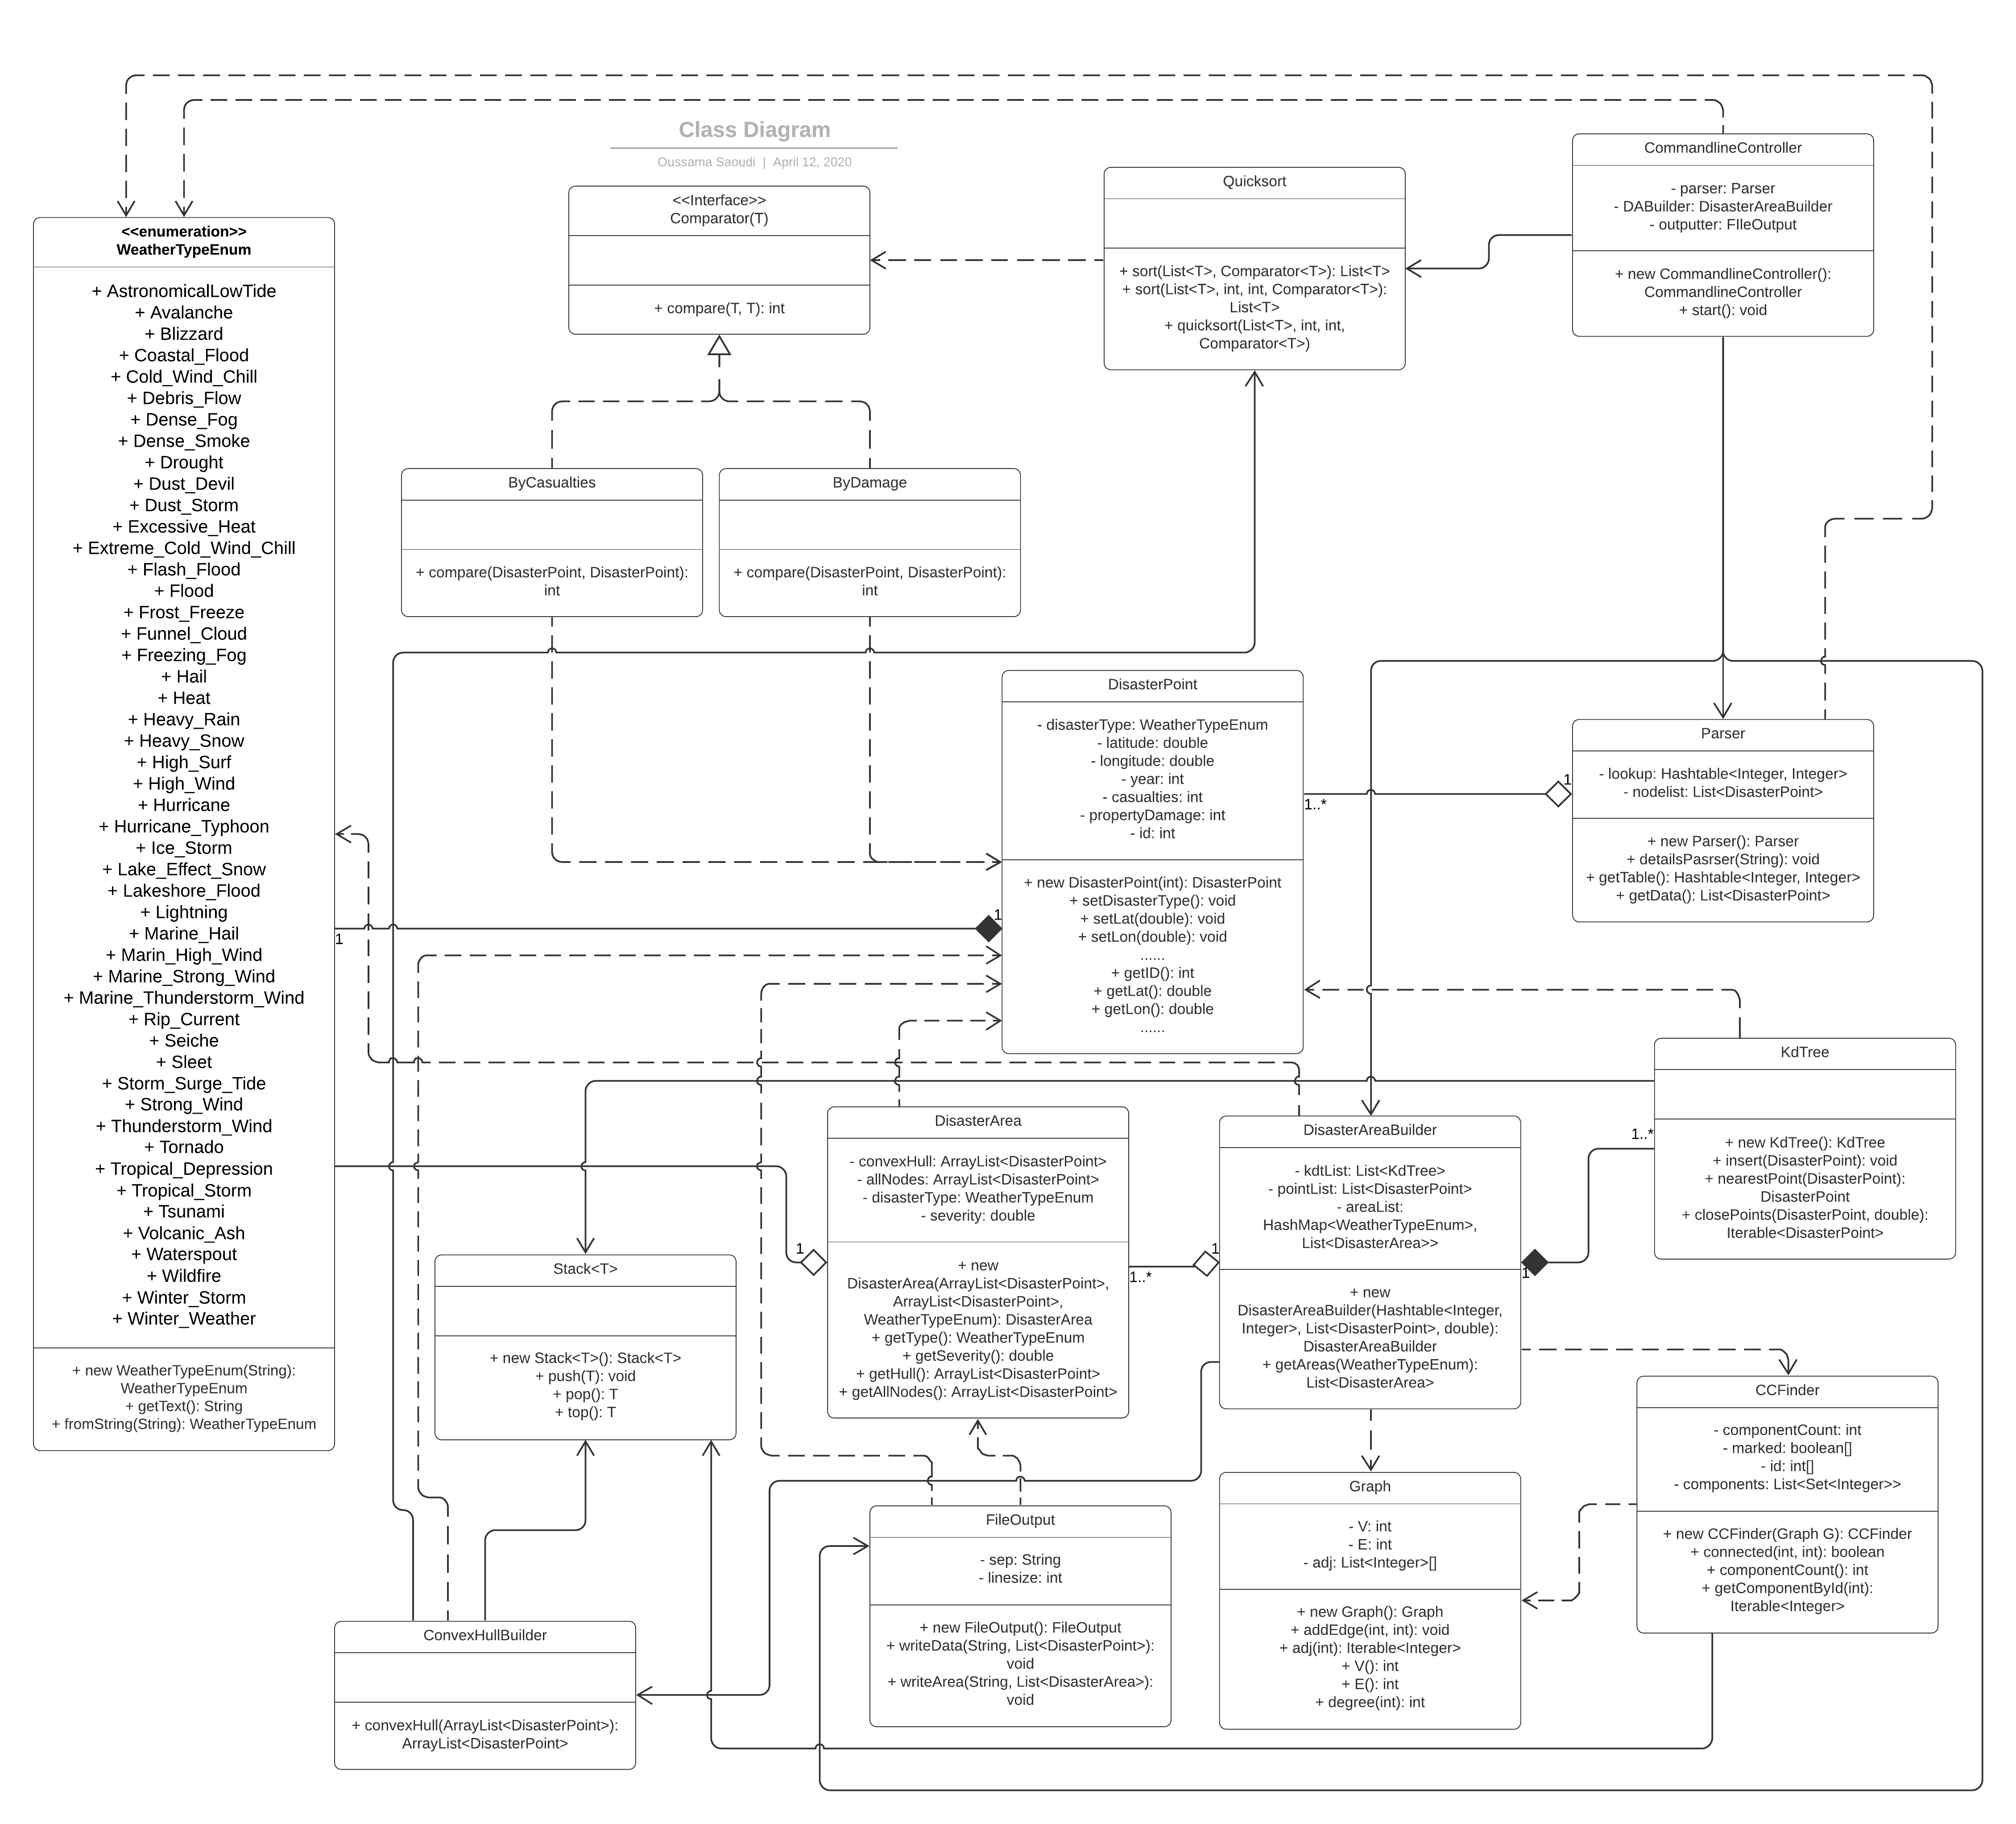
\includegraphics[scale=0.5]{UML_Class_Diagram.png}
            \caption{UML Class Diagram for Project Vayu}
            \label{fig:my_label}
        \end{figure}
                
        \subsection{Algorithm viewpoint}
            The algorithms that were used in this software was Graph, DepthFirstSearch,Quicksort,KdTree
            \subsubsection{Design concerns}
                \paragraph{QuickSort} Quicksort is a sorting algorithm with a typical performance of $Nlg(N)$ and a worst case performance of
                $O(N^2)$ for an array of size $N$. Typically Quicksort is in place, but the implementation used makes a copy of the
                array and then sorts it, which leads to extra space of $O(N)$\\
                
                \paragraph{Graph} A graph is used in the implementation. A graph is created with nodes size of V and has E edges added to it. Upon initializing the graph takes a time of $O(V)$ to do. Adding an edge is constant time $O(1)$, and doing so E times will result in overall 
                performance in constructing the graph to be $O(V + E)$. The extra space used by the Graph is used to store an adjacency list,
                which takes a space of $O(V+E)$\\
                
                \paragraph{Connected Component Finder} CCFinder is a module which uses depth first search to  is an algorithm used to traverse a graph and assign elements to their respective connected component. Depth First search analyzes each edge and each vertex once, thus having a performance of $O(V + E)$. CCFinder also stores a list of all the connected components, which uses extra space proportional to $O(V)$\\
                
                \paragraph{KdTree} Finding the nearest point only takes $O(lg(N))$ in typical cases, but can reach a performance of $O(N)$ in the worst case. For range, it depending on how dense the graph is, the performance can also be between $O(lg(N))$ and $O(N)$. The space that the KdTree takes is an additional $O(N)$ for representing each node in the tree and a rectangle which represents the space the node is a root for.\\
                
                \paragraph{Convex Hull} The ConvexHullBuilder constructs a convex hull out of a list of points. A convex hull is the smallest set of points such that when a polygon is made from the points it covers all points and edges between them. The algorithm used to construct the convex hull builder is the Graham Scan, which uses the quick sort algorithm for a performance of $O(NlgN))$ for an input set of size $N$. The ConvexHuLLBuilder creates a new array using the created sorting algorithm, so the extra space used is $O(N)$.
            \subsubsection{Design elements}
                Each algorithm has it's own module by the same name.
            \subsection{Processing Attributes} 
                \paragraph{Quicksort} Quick sort works by partitioning a given list with a pivot element, and putting all lesser elements to the left of the element, and all greater elements on the right of the pivot element. Then, it recursively sorts the two subsections on either side of the pivot element. The pivot element is chosen by randomly choosing an element from all the elements in the list. Quicksort can also have the lowest and highest indices defined for the sort to sort only a subsection of the algorithm.
                \paragraph{Graph} The graph is made by creating an array of $ArrayList<Integer>$, where each of the lists represents the adjacent vertices for a vertex. An integer vertex's adjacency list can be found at its integer position at the array of $ArrayList<Integer>$. Additing an edge adds the vertex to both of the ArrayLists of the vertices. Parallel and self loop edges are allowed in the Graph model used.
                \paragraph{Connected Component Finder} The connected component finder works by creating an array of booleans called marked, which shows whether each vertex has been visited by the dfs yet. Then, CCFinder goes through each vertex in order of their values, performing dfs at each vertex that is not yet marked. When dfs is run on a source vertex, it is added to a Stack, and then enters a loop. In the loop the stack is popped, the vertex is added to that connected component, and all the popped vertex's adjacent vertices are added to the Stack if they haven't been marked, and are marked. This continues until the stack is empty. Once the dfs returns, the number of connected components is increased. And the loop continues until all vertices are marked. This supports constant time return of connected components.
                \paragraph{KdTree} A KdTree is a binary tree datastructure representing points in 2d space, allowing for quick insertion of nodes as well as quick retrieval of information such as finding the nearest neighbor and finding all points which reside inside a rectangular area. The KdTree is constructed as follows: All the even valued levels in the binary tree have nodes with a vertical orientation, meaning that all nodes to its left are spatially to its left, and all nodes in the right branch are spatially to its right or on the dividing line. All the odd valued levels in the binary tree have nodes with horizontal orientation, meaning that all nodes to the left subtree are spatially below the point, and all nodes to the right subtree are spatially above or on the dividing line. Additionally every node contains a rectangle which contains all the nodes contained in the node's subtree. Insertion simply works like binary search in that if a node is to the "left" then it goes down to that branch until it hits a null value and returns a reference to a leaf node. In searching for nearest neighbor, the KdTree progressively improves its estimate of the nearest neighbor as it searches for the value in its subtree. If the distance to the node is closer to the dividing line of the node than to the nearest node, the opposite subtree must also be explored. The range function explores the tree looking for points which intersect with a given rectangular range. It does so by recursively checking both sides. The cases are as follows: if the node's left rectangle intersects with the searched rectangle, then it calls range on the node's left child. If the node's right rectangle intersects with the searched rectangle, then it calls range on the node's right child. if the rectangle ever intersects with the node's point, then add the point to a stack to save the points that are within the range.
                \paragraph{Convex Hull} The convex hull algorithm used is the Graham scan algorithm which works as follows: First find the point with the minimum y value, and break ties by choosing the one with the minimum x value. Set that point as the anchor. Then sort all the points in the input list by comparing their radial angles from the x axis relative to the anchor, with lowest angle to x axis being at the beginning. Then go through and add the points one by one, adding them to the stack. For each point added, check that the orientation of the next-to-top node of the stack, the top node of the stack, and the next point to be added is not clockwise. While it is the case, pop the top element of the stack. Then, add the point to the stack. Once all points have been analyzed the Stack will contain all the points that are supposed to be on the convex hull. If there are fewer than three points, return null because a convex hull must have at minimum 3 points. Else return the stack or transfer the nodes on the stack to an ArrayList (As done in this software implementation).
                

%\section{Design Overlays}
\section{Design Rationale}
    An object-oriented approach during the design process allowed for efficient division of the workload between group members, and an overall simpler design that allowed for a fairly simple integration of components. The design rationale shall be discussed for the following six subsections:
    \paragraph{Sorting} The sorting algorithm used is quicksort, which is used to fulfill the requirement FR[1.1]. The algorithm was chosen for its fast linearithmic performance as well as its in-place nature, which makes it much more space efficient than the alternative mergesort. The speed of quicksort was of utmost importance in order to meet the functional requirement FR[4.1]
    
    \paragraph{Disaster Areas} To fulfill functional requirement FR[2.1], a method was needed to find proximal points of the same type, aggregate them, and create areas which represent areas affected by a type of natural disaster. To find the proximal points, a KdTree was used because of its typical logarithmic performance of finding proximal points. To aggregate points, it was decided to use a graph to represent points, edges to represent sufficient proximity, and connected components to represent the aggregation of all the proximal points. The connected components contains all the DisasterPoints which are contained in an area. The algorithm used to find the connected components was a simple depth first search variant which marked the connected components of every node. It utilized already made Stack code, and is able to find the connected components in optimal time, which is proportional to the number of vertices and edges. Finally, to fully fulfill FR[2.1] a convex hull algorithm needed to be used to compute the convex hull of the connected component. The algorithm chosen was the Graham Scan for its simplicity of implementation, its use of already implemented code (namely, quick sort), and its linearithmic performance.
  
    \paragraph{Parser} Due to the input data, there were several fields describing indirect and direct injury and death as a result of the disaster. It was decided to represent casualties by the sum of all these values and to store that into the DisasterPoint data type. The input data also had many unfilled fields throughout the files. It was decided to retain these fields and set unused values to either null or 0 to retain whatever information the DisasterPoint does have instead of discarding it. However, any line that did not contain a longitude and latitude would not be created into a DisasterPoint and the data was instead discarded. This is because latitude and longitude values are integral to the system working, namely in the DisasterAreaBuilder module. Finally, the decision to only parse StormEvent Details is due to the fact that the file contains all the information needed by the system, and so the additional information files were not parsed or used by the program.
    
    \paragraph{Output} In order to make the output user friendly as well, as outlined on FR[4.2], it was decided to prioritize readability of the output file so that values are presented in a table on the output file instead of making the file a CSV file. The output file will always be a text file output by java, thus satisfying FR[3.1]
    
    \paragraph{Commandline Interface} The decision to use a command line interface stems primarily from ease of implementation and the short time it takes to build a good one, which allows for development under the time constraint. The commandline interface is designed to provide help to the user through helpful tips on how to use it, which assists in fulfilling FR[4.2]
    
    \paragraph{Overall Design} An important decision made with the overall design is to create a list of disaster points and a lookup table and pass references to them the primary controlling methods, namely DisasterAreaBuilder and CommandlineController. The use of both a list and a lookup table is to allow for constant time operation of getting the index representation of a DisasterPoint and getting a DisasterPoint from its index. An example of use of the lookup table is inserting edges into the graph in DisasterAreaBuilder, where the DisasterPoints were known but the index versions of the node were needed to insert edges into the graph. An example of the use of the DisasterPoints list is in passing the reference for sorting in CommandlineController, as well as converting integer points into DisasterPoints such as when the connected components were retrieved from the graph implementation in DisasterAreaBuilder.
%\section{Review}%design review

\section*{State machines}
\subsection*{DisasterAreaBuilder}  
\newpage
\begin{figure}
            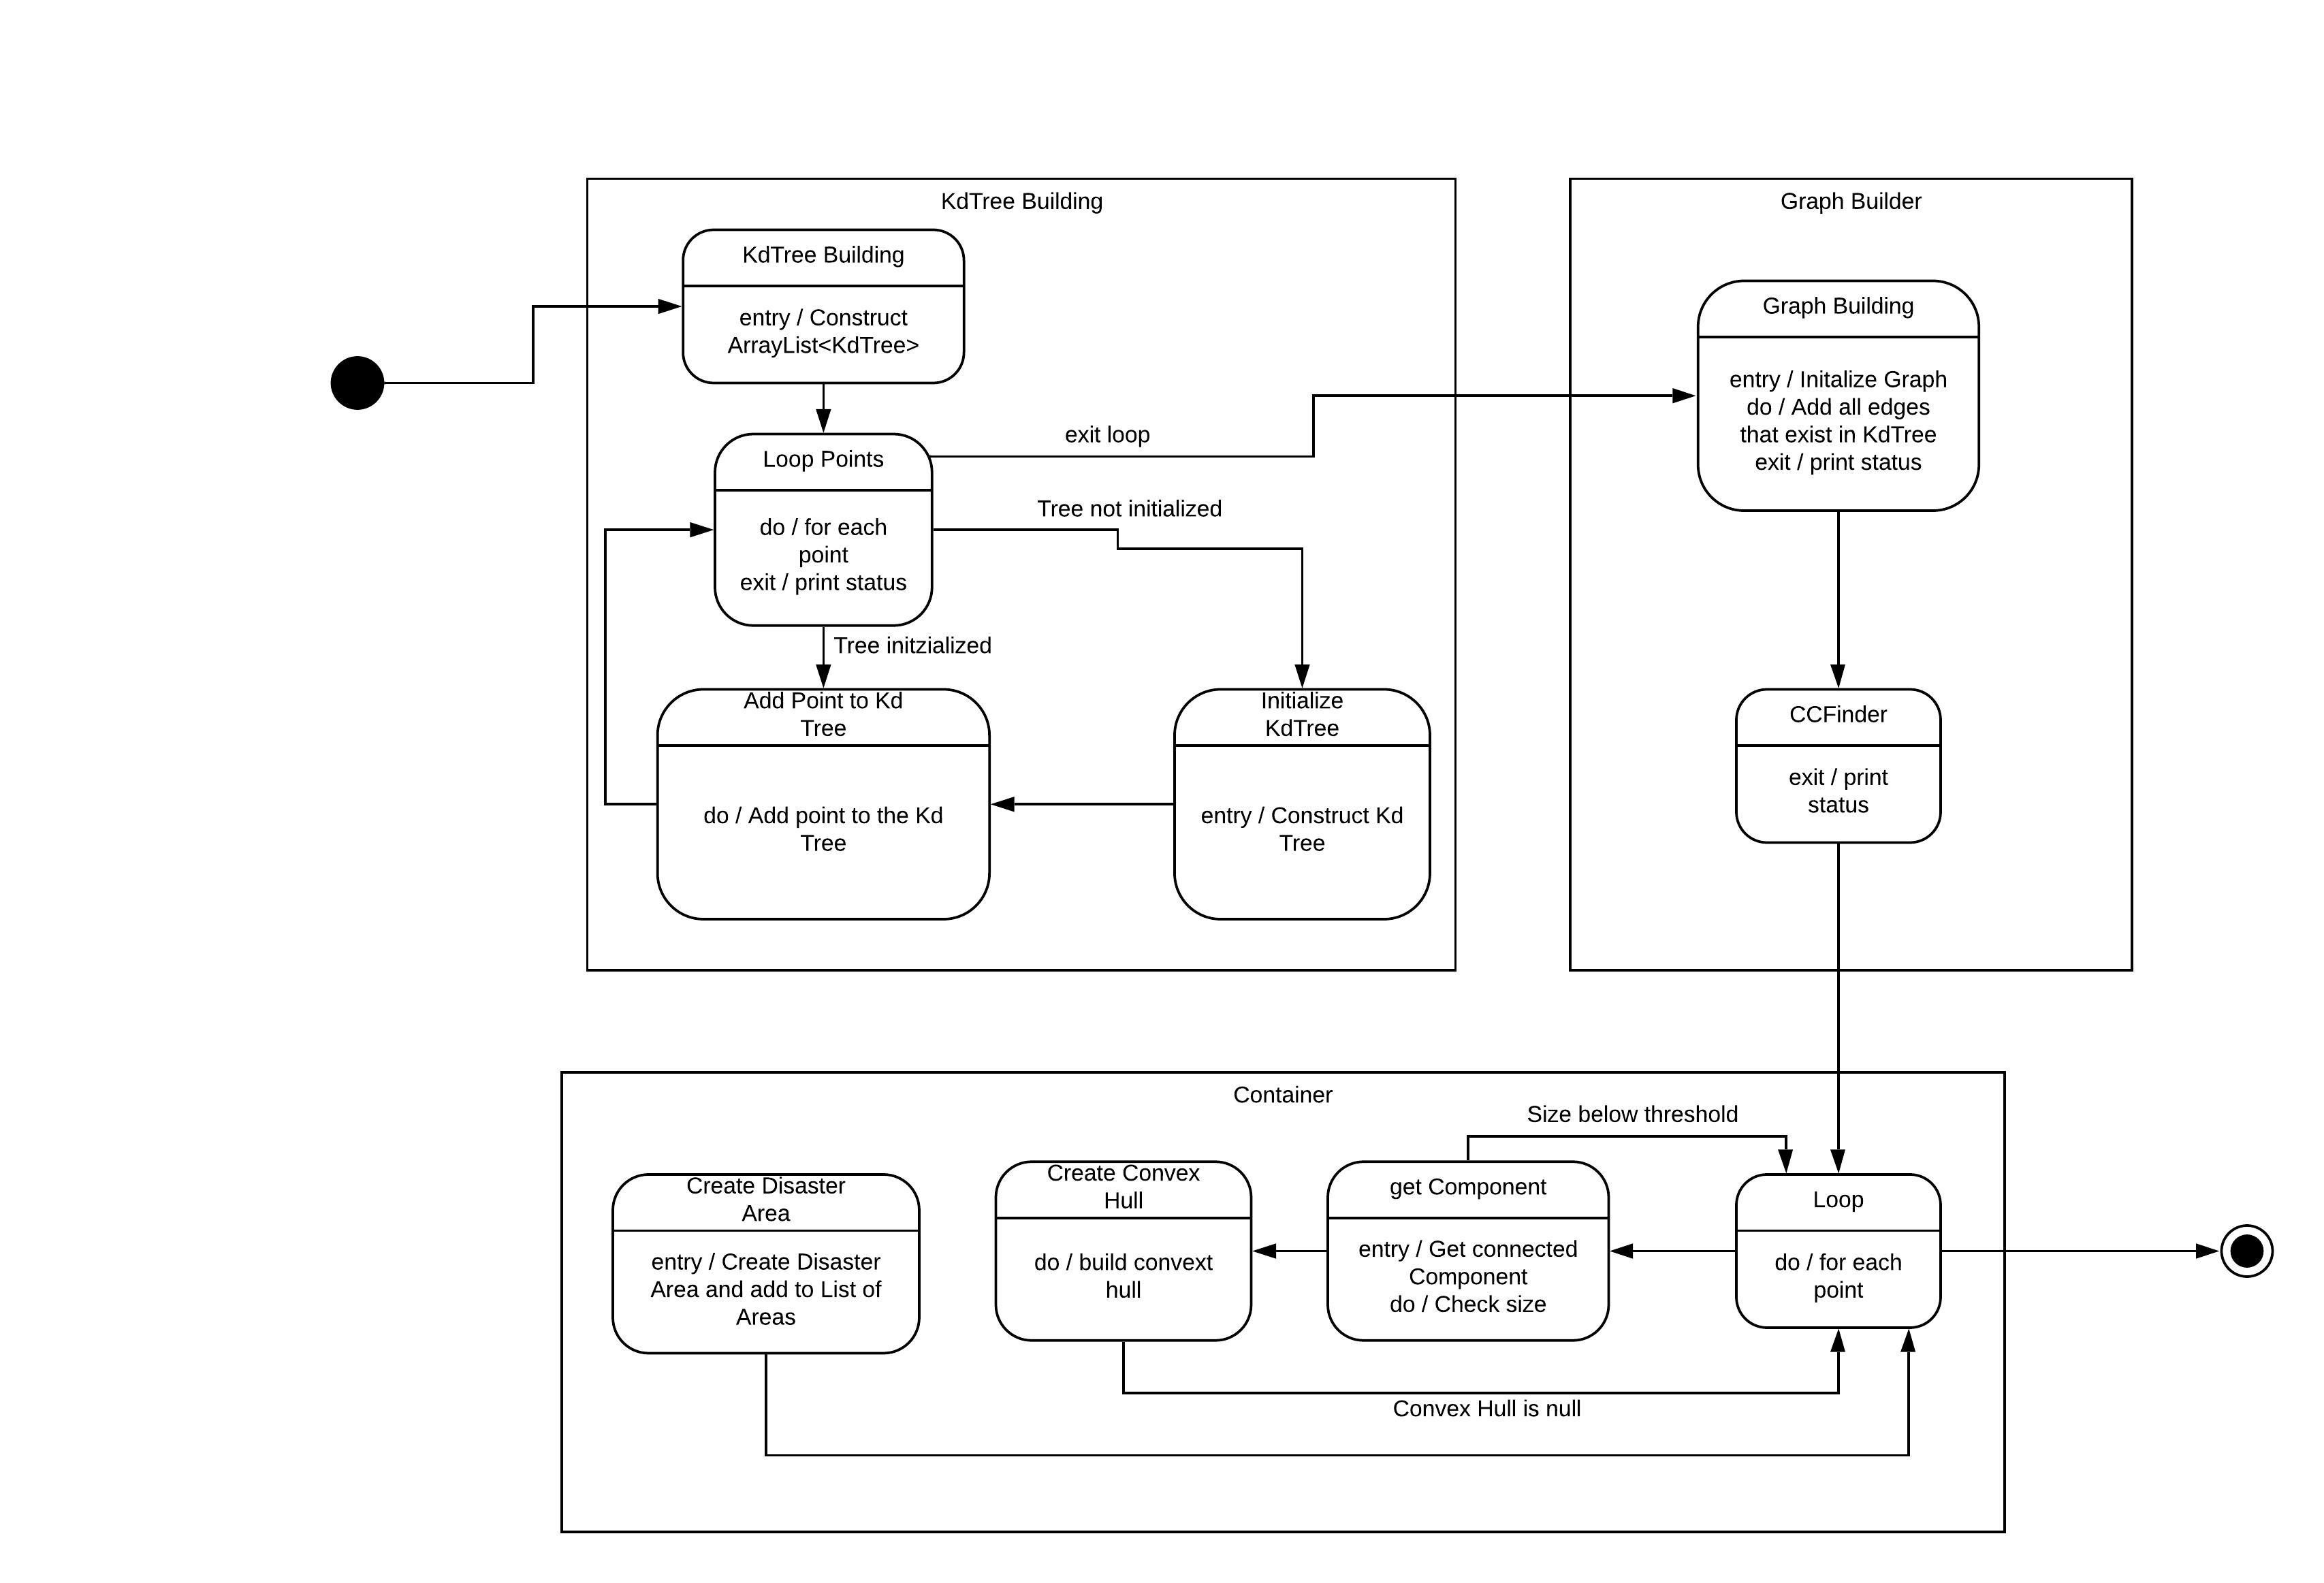
\includegraphics[scale=0.5]{State_Machine_DisasterAreaBuilder.jpeg}
            \caption{UML State Diagram for DisasterAreaBuilder}
            \label{fig:state_one}
\end{figure}
\begin{figure}
            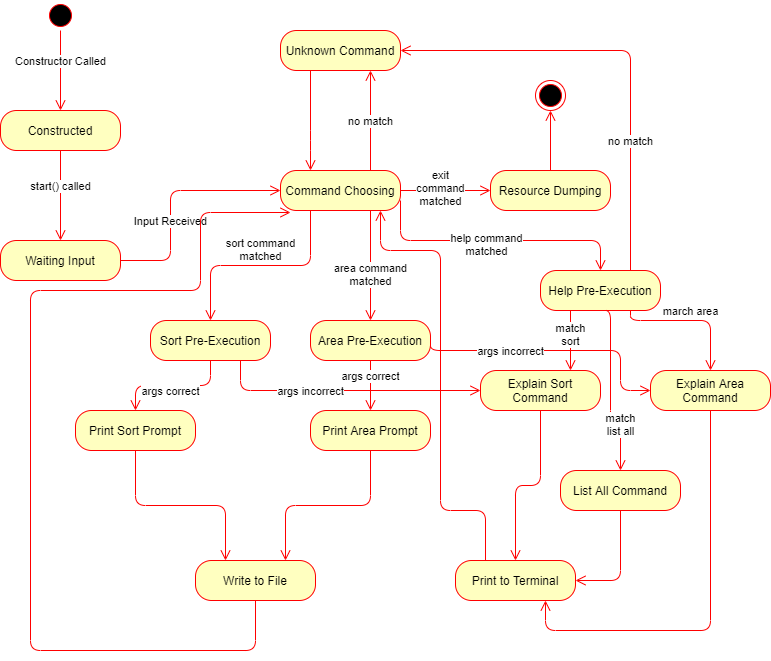
\includegraphics[scale=0.5]{State_Diagram_CLC.png}
            \caption{UML State Diagram for CommandlineController}
            \label{fig:state_two}
\end{figure}

\normalsize
\end{document}
% a description of the classes/modules you have decided to use in your application, and your explanation of why you have decomposed the application into those classes; You should include a UML class diagram showing a static representation of your application classes and relationship between classes; 

% for each class, a description of the interface (public entities), and make sure that there is a description of the semantics (behaviour) of each public method in the class, as well as a description of the syntax

% a view of the uses relationship;

% include a trace back to requirements in each class interface;

% for each class, a description of the implementation (private entities), including class variables - include enough detail to show how the class variables are maintained by the methods in the class; you should include two UML state machine diagrams for two most interesting classes in your implementation; 

%  an internal review/evaluation of your design.